\documentclass[11pt,preprint, authoryear]{elsarticle}

\usepackage{lmodern}
%%%% My spacing
\usepackage{setspace}
\setstretch{1.2}
\DeclareMathSizes{12}{14}{10}{10}

% Wrap around which gives all figures included the [H] command, or places it "here". This can be tedious to code in Rmarkdown.
\usepackage{float}
\let\origfigure\figure
\let\endorigfigure\endfigure
\renewenvironment{figure}[1][2] {
    \expandafter\origfigure\expandafter[H]
} {
    \endorigfigure
}

\let\origtable\table
\let\endorigtable\endtable
\renewenvironment{table}[1][2] {
    \expandafter\origtable\expandafter[H]
} {
    \endorigtable
}


\usepackage{ifxetex,ifluatex}
\usepackage{fixltx2e} % provides \textsubscript
\ifnum 0\ifxetex 1\fi\ifluatex 1\fi=0 % if pdftex
  \usepackage[T1]{fontenc}
  \usepackage[utf8]{inputenc}
\else % if luatex or xelatex
  \ifxetex
    \usepackage{mathspec}
    \usepackage{xltxtra,xunicode}
  \else
    \usepackage{fontspec}
  \fi
  \defaultfontfeatures{Mapping=tex-text,Scale=MatchLowercase}
  \newcommand{\euro}{€}
\fi

\usepackage{amssymb, amsmath, amsthm, amsfonts}

\def\bibsection{\section*{References}} %%% Make "References" appear before bibliography


\usepackage[round]{natbib}

\usepackage{longtable}
\usepackage[margin=2.3cm,bottom=2cm,top=2.5cm, includefoot]{geometry}
\usepackage{fancyhdr}
\usepackage[bottom, hang, flushmargin]{footmisc}
\usepackage{graphicx}
\numberwithin{equation}{section}
\numberwithin{figure}{section}
\numberwithin{table}{section}
\setlength{\parindent}{0cm}
\setlength{\parskip}{1.3ex plus 0.5ex minus 0.3ex}
\usepackage{textcomp}
\renewcommand{\headrulewidth}{0.2pt}
\renewcommand{\footrulewidth}{0.3pt}

\usepackage{array}
\newcolumntype{x}[1]{>{\centering\arraybackslash\hspace{0pt}}p{#1}}

%%%%  Remove the "preprint submitted to" part. Don't worry about this either, it just looks better without it:
\makeatletter
\def\ps@pprintTitle{%
  \let\@oddhead\@empty
  \let\@evenhead\@empty
  \let\@oddfoot\@empty
  \let\@evenfoot\@oddfoot
}
\makeatother

 \def\tightlist{} % This allows for subbullets!

\usepackage{hyperref}
\hypersetup{breaklinks=true,
            bookmarks=true,
            colorlinks=true,
            citecolor=blue,
            urlcolor=blue,
            linkcolor=blue,
            pdfborder={0 0 0}}


% The following packages allow huxtable to work:
\usepackage{siunitx}
\usepackage{multirow}
\usepackage{hhline}
\usepackage{calc}
\usepackage{tabularx}
\usepackage{booktabs}
\usepackage{caption}


\newenvironment{columns}[1][]{}{}

\newenvironment{column}[1]{\begin{minipage}{#1}\ignorespaces}{%
\end{minipage}
\ifhmode\unskip\fi
\aftergroup\useignorespacesandallpars}

\def\useignorespacesandallpars#1\ignorespaces\fi{%
#1\fi\ignorespacesandallpars}

\makeatletter
\def\ignorespacesandallpars{%
  \@ifnextchar\par
    {\expandafter\ignorespacesandallpars\@gobble}%
    {}%
}
\makeatother

\newlength{\cslhangindent}
\setlength{\cslhangindent}{1.5em}
\newenvironment{CSLReferences}%
  {\setlength{\parindent}{0pt}%
  \everypar{\setlength{\hangindent}{\cslhangindent}}\ignorespaces}%
  {\par}


\urlstyle{same}  % don't use monospace font for urls
\setlength{\parindent}{0pt}
\setlength{\parskip}{6pt plus 2pt minus 1pt}
\setlength{\emergencystretch}{3em}  % prevent overfull lines
\setcounter{secnumdepth}{5}

%%% Use protect on footnotes to avoid problems with footnotes in titles
\let\rmarkdownfootnote\footnote%
\def\footnote{\protect\rmarkdownfootnote}
\IfFileExists{upquote.sty}{\usepackage{upquote}}{}

%%% Include extra packages specified by user

%%% Hard setting column skips for reports - this ensures greater consistency and control over the length settings in the document.
%% page layout
%% paragraphs
\setlength{\baselineskip}{12pt plus 0pt minus 0pt}
\setlength{\parskip}{12pt plus 0pt minus 0pt}
\setlength{\parindent}{0pt plus 0pt minus 0pt}
%% floats
\setlength{\floatsep}{12pt plus 0 pt minus 0pt}
\setlength{\textfloatsep}{20pt plus 0pt minus 0pt}
\setlength{\intextsep}{14pt plus 0pt minus 0pt}
\setlength{\dbltextfloatsep}{20pt plus 0pt minus 0pt}
\setlength{\dblfloatsep}{14pt plus 0pt minus 0pt}
%% maths
\setlength{\abovedisplayskip}{12pt plus 0pt minus 0pt}
\setlength{\belowdisplayskip}{12pt plus 0pt minus 0pt}
%% lists
\setlength{\topsep}{10pt plus 0pt minus 0pt}
\setlength{\partopsep}{3pt plus 0pt minus 0pt}
\setlength{\itemsep}{5pt plus 0pt minus 0pt}
\setlength{\labelsep}{8mm plus 0mm minus 0mm}
\setlength{\parsep}{\the\parskip}
\setlength{\listparindent}{\the\parindent}
%% verbatim
\setlength{\fboxsep}{5pt plus 0pt minus 0pt}



\begin{document}



\begin{frontmatter}  %

\title{Question 3: Portfolio Construction}

% Set to FALSE if wanting to remove title (for submission)




\author[Add1]{Andrew Hyde}
\ead{}







\begin{abstract}
\small{
Abstract to be written here.
}
\end{abstract}

\vspace{1cm}





\vspace{0.5cm}

\end{frontmatter}



%________________________
% Header and Footers
%%%%%%%%%%%%%%%%%%%%%%%%%%%%%%%%%
\pagestyle{fancy}
\chead{}
\rhead{}
\lfoot{}
\rfoot{\footnotesize Page \thepage}
\lhead{}
%\rfoot{\footnotesize Page \thepage } % "e.g. Page 2"
\cfoot{}

%\setlength\headheight{30pt}
%%%%%%%%%%%%%%%%%%%%%%%%%%%%%%%%%
%________________________

\headsep 35pt % So that header does not go over title




\hypertarget{introduction}{%
\section{\texorpdfstring{Introduction
\label{Introduction}}{Introduction }}\label{introduction}}

Using the information on the ALSI (J200) and SWIX (J400) top 40 Indexes,
write a brief research report in Texevier where you:

Compare the SWIX and ALSI methodologies by looking at the performance of
different size indexes (large, mid and small caps), sector exposures and
stock concentration over time. Use your discretion in writing a short
report highlighting differences in the return profiles

\hypertarget{the-data}{%
\section{The Data}\label{the-data}}

I make use of the function from the practical to impute missing returns

\hypertarget{stratification-of-idexes}{%
\section{Stratification of Idexes}\label{stratification-of-idexes}}

You may use stratification of data/usdzar.rds to provide insight into
the different return profiles of both methodologies during different
periods of currency performance and volatility.

Here I reply on the courses practical notes. I begin by creating the
index returns using this capped weight estimator using the tbl2xts
framework. Begin by plotting the culumative returns for each index.

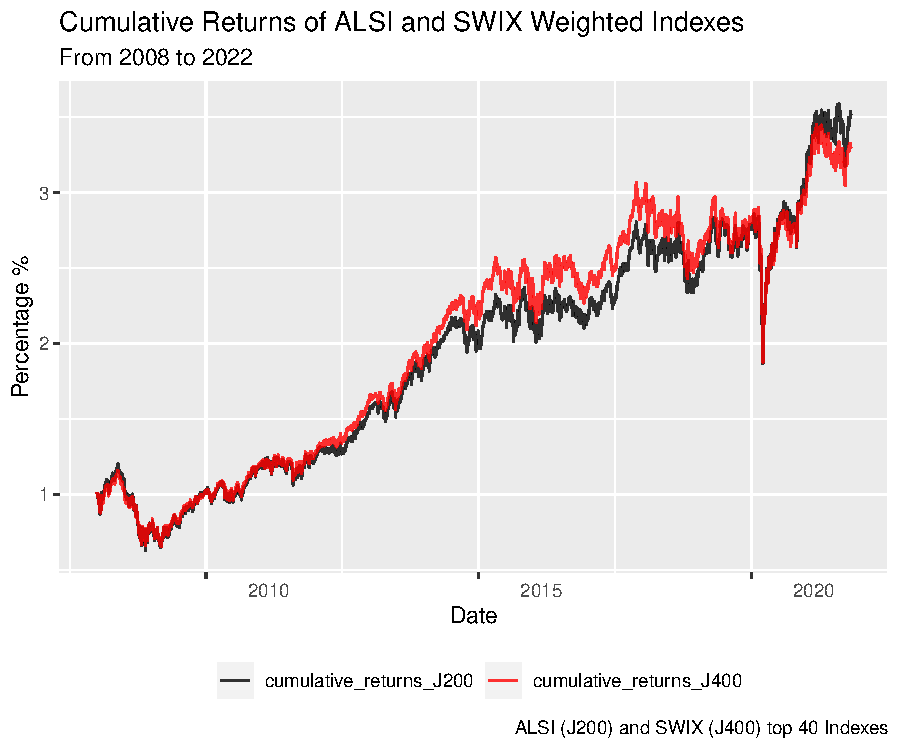
\includegraphics{Question3_files/figure-latex/unnamed-chunk-2-1.pdf}

Break down cumulative returns by industry

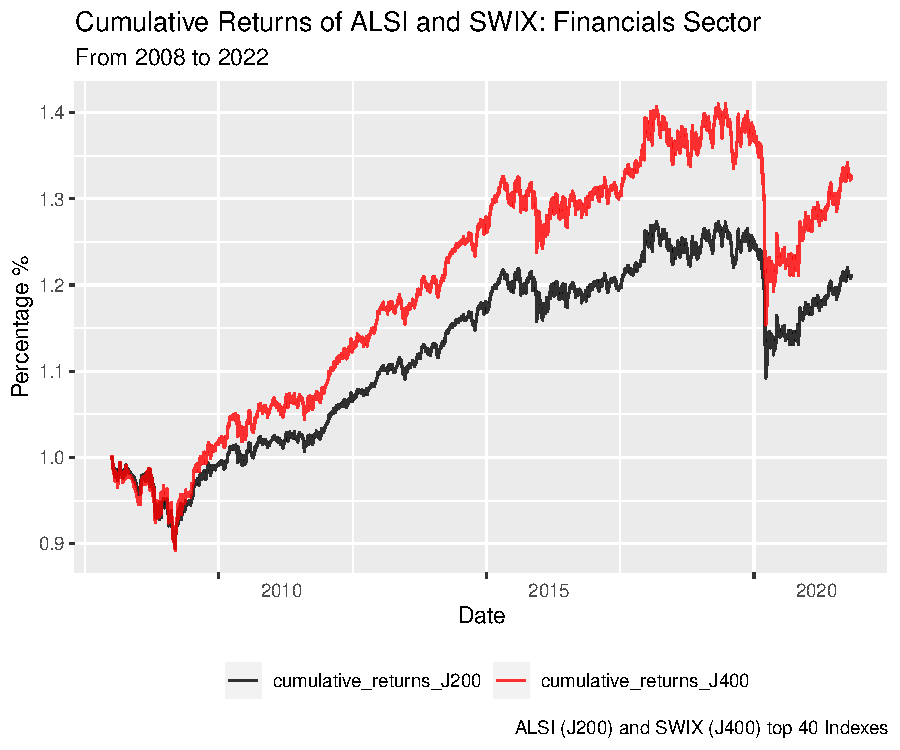
\includegraphics{Question3_files/figure-latex/unnamed-chunk-3-1.pdf}

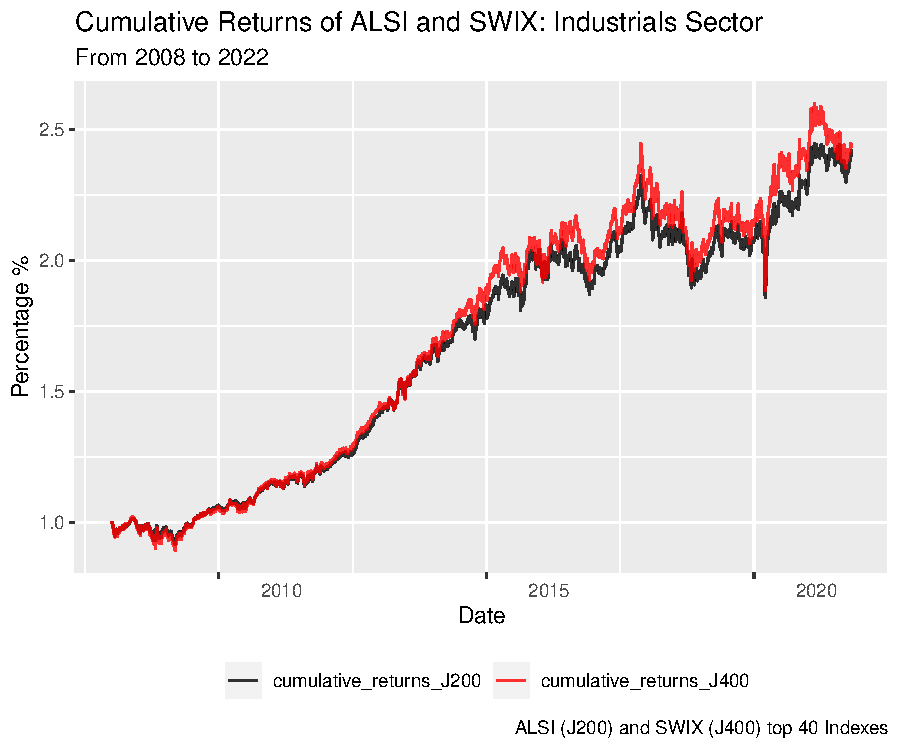
\includegraphics{Question3_files/figure-latex/unnamed-chunk-4-1.pdf}

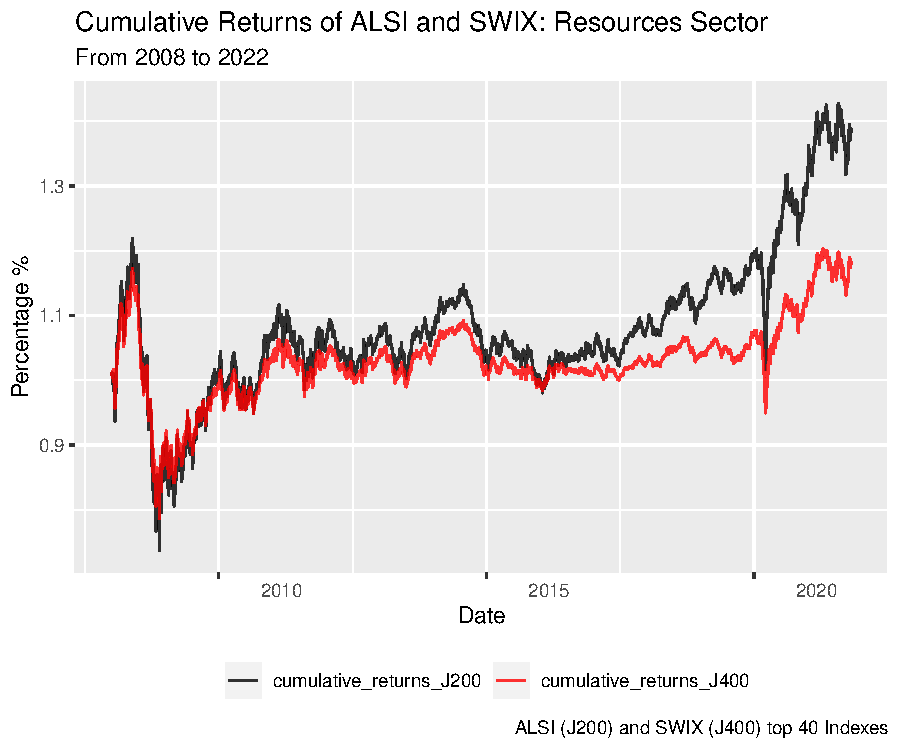
\includegraphics{Question3_files/figure-latex/unnamed-chunk-5-1.pdf}

\hypertarget{capping-indexes}{%
\section{Capping Indexes}\label{capping-indexes}}

Answer the JSE's question on applying capping to the indexes - in
particular looking at the impact different capping levels would have had
on both the SWIX and ALSI (6\% and 10\%). Use data/Rebalance days.rds to
identify the Rebalance Days during past quarterly rebalances.

\begin{verbatim}
##       date    Tickers Short.Name     Return     Sector Index_Name       J400 
##          0          0          0          0          0       1239       2004 
##       J200 
##       1720
\end{verbatim}

\begin{verbatim}
## # A tibble: 40 x 5
##    date       Tickers       weight RebalanceTime   sum
##    <date>     <chr>          <dbl> <chr>         <dbl>
##  1 2008-03-20 AGL SJ Equity 0.100  2008March         1
##  2 2008-03-20 BHP SJ Equity 0.0821 2008March         1
##  3 2008-03-20 SOL SJ Equity 0.0390 2008March         1
##  4 2008-03-20 MTN SJ Equity 0.0385 2008March         1
##  5 2008-03-20 CFR SJ Equity 0.0351 2008March         1
##  6 2008-03-20 IMP SJ Equity 0.0307 2008March         1
##  7 2008-03-20 SAB SJ Equity 0.0290 2008March         1
##  8 2008-03-20 SBK SJ Equity 0.0195 2008March         1
##  9 2008-03-20 AMS SJ Equity 0.0183 2008March         1
## 10 2008-03-20 REM SJ Equity 0.0147 2008March         1
## # ... with 30 more rows
## # i Use `print(n = ...)` to see more rows
\end{verbatim}

\bibliography{Tex/ref}





\end{document}
